\documentclass{mp}
\usepackage{bm}
\newcommand{\dd}[1]{\partial#1}
\graphicspath{{10_korelacja}}
\subtitle{Momenty dwuwymiarowe}
\DeclareMathOperator{\cov}{cov}
\begin{document}
\frame{\titlepage}
\begin{frame}{Momenty zmiennych losowych}
\begin{block}{Moment rzędu $l$ względem punktu $c$}
\[ E(X-c)^l=\begin{cases} \sum_{x_i} (x_i-c)^lp_i & $X$\text{ typu skokowego} \\
\int_{-\infty}^\infty (x-c)^lf(x)\d{x} & $X$\text{ typu ciągłego}
\end{cases} \]
\end{block}
\begin{description}
\item[moment zwykły] $c=0$
\item[moment centralny] $c=\mu$
\end{description}
\end{frame}
\begin{frame}{Momenty dwuwymiarowe}
\begin{description}
\item<+->[moment zwykły rzędu $l+r$] \[E(X^lY^r)\]
\item<+->[moment centralny rzędu $l+r$] \[E((X-EX)^l(Y-EY)^r)\]
\item<+->[kowariancja] \[\cov(X,Y)=E((X-EX)(Y-EY))=EXY-EXEY\]
\end{description}
\only<+->
{
\begin{block}{Twierdzenie}
\[\left(\forall x,y\in\R\colon P(X<x,Y<y)=P(X<x)P(Y<y) \right) \alert{\to} cov(X,Y)=0 \]
\end{block}
}
\end{frame}
\begin{frame}{Współczynnik korelacji}
\[\varrho=\frac{\cov(X,Y)}{\sigma_X\sigma_Y} \]
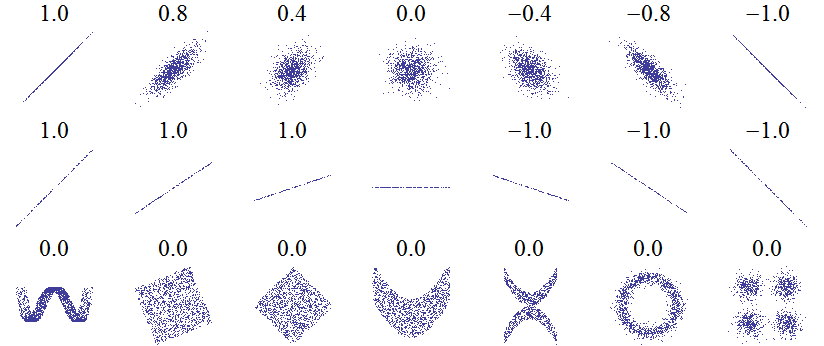
\includegraphics[width=\textwidth]{10_korelacja/Correlation_examples.png}

{\tiny \url{http://upload.wikimedia.org/wikipedia/commons/0/02/Correlation_examples.png} domena publiczna}
\end{frame}
\begin{frame}{Podejrzane korelacje}
\url{http://tylervigen.com/}
\end{frame}

\begin{frame}{Momenty warunkowe}
\only<1>
{
\begin{block}{Zmienne dyskretne}
\begin{gather*}
E((X-c)^l|Y=y_j)=\sum_{x_i} (x_i-c)^lP(X=x_i|Y=y_j)=\sum_{x_i} (x_i-c)^l\frac{p_{i,j}}{p_{\cdot,j}} \\
E(X|Y=y_j)=\frac{1}{p_{\cdot,j}}\sum_{x_i} x_ip_{i,j} \\
\end{gather*}
\end{block}
}
\only<2>
{
\begin{block}{Zmienne typu ciągłego}
\begin{gather*}
E((X-c)^l|Y=y)=\int_{-\infty}^\infty (x-c)^lf(x|y)\d{x}=\int_{-\infty}^\infty (x-c)^l\frac{f(x,y)}{f_Y(y)}\d{x} \\
E(X|Y=y)=\frac{1}{f_Y(y)}\int_{-\infty}^\infty xf(x,y)\d{x}
\end{gather*}
\end{block}
}
\only<3>
{
\begin{block}{Wariancja warunkowa}
\[ D^2(X|Y=y)=E\left[(X-E(X|Y=y))^2|Y=y\right] \]
\end{block}
}
\end{frame}

\begin{frame}{Krzywe regresji}
\begin{block}{Regresja I rodzaju}
\[ r(x)=E(Y|X=x)  \]
\note{Jeżeli zmienne są niezależne, to $E(Y|X=x)=EY$. Dla zmiennych dyskretnych może wyjść śmieszna sieczka.}
\end{block}
\pause
\begin{block}{Regresja II rodzaju}
\[ r(x)=ax+b \qquad E\left[Y-r(X)\right]^2\to\min \]
\note
{
	\begin{gather*}
	f(a,b)=E(Y-(aX+b))^2\to\min \implies f'(a,b)=\bm{0} \\
	f(a,b)=E(Y^2+(aX+b)^2-2Y(aX+b))\\
	f(a,b)=E(Y^2+a^2X^2+2abX+b^2-2aXY-2bY)\\
	f(a,b)=EY^2+a^2EX^2+2abEX+b^2-2aEXY-2bEY \\
	\frac{\dd{f(a,b)}}{\dd{a}}=2aEX^2+2bEX-2EXY=0 \\
	\frac{\dd{f(a,b)}}{\dd{b}}=2aEX+2b-2EY=0 \\
	b=EY-aEX \\
	aEX^2+bEX-EXY=0 \\
	aEX^2+(EY-aEX)EX-EXY=0 \\
	aEX^2+EXEY-aE^2X-EXY=0 \\
	a=\frac{EXY-EXEY}{EX^2-E^2X}=\frac{\cov(X,Y)}{D^2X} \\
	\end{gather*}
}
\pause
\[ a=\frac{\cov(X,Y)}{D^2X} \qquad b=EY-aEX \]
\end{block}
\end{frame}

\begin{frame}{Wektory zmiennych losowych $(X_1,X_2,\ldots,X_n)$}
\[ \bm{\mu}=\begin{bmatrix} \mu_1 \\ \mu_2 \\ \vdots \\ \mu_n \end{bmatrix} \]
\[ \Sigma=\begin{bmatrix}
\cov(X_1,X_1) & \cov(X_1,X_2) & \ldots & \cov(X_1,X_n) \\
\cov(X_2,X_1) & \cov(X_2,X_2) & \ldots & \cov(X_2,X_n) \\
\vdots & \vdots & \ddots & \vdots \\
\cov(X_n,X_1) & \cov(X_n,X_2) & \ldots & \cov(X_n,X_n) \\
\end{bmatrix} \]
\end{frame}


%\item<+->[wektor wartości średnich] \[\mathbf{\mu}=\begin{pmatrix}\mu_{1,0}\\\mu_{0,1}\end{pmatrix}\only<+->{=\begin{pmatrix}\mu_X\\\mu_Y\end{pmatrix}}\]
%\item<+->[macierz kowariancji] \[\Sigma=\begin{bmatrix}\sigma_{2,0} & \sigma_{1,1} \\ \sigma_{1,1} & \sigma_{0,2} \end{bmatrix}\]
\end{document}
